\section{Background}
\subsection{Looplets}
Finch represents iteration patterns using Looplets, a language that decomposes datastructure iterators hierarchically. Looplets represent the control-flow structures needed to iterate over any given datastructure, or multiple datastructures simultaneously. In particular, looplets are good at lifting code to the highest loop level that it's needed and subdividing iteration hierarchically in coordinate space. Because looplets are compiled with progressive lowering, structure-specific mathematical optimizations such as integrals, multiply by zero, etc. can be implemented using simple compiler passes like term rewriting and constant propagation.

We begin a formal description of looplets here:

\begin{figure}
	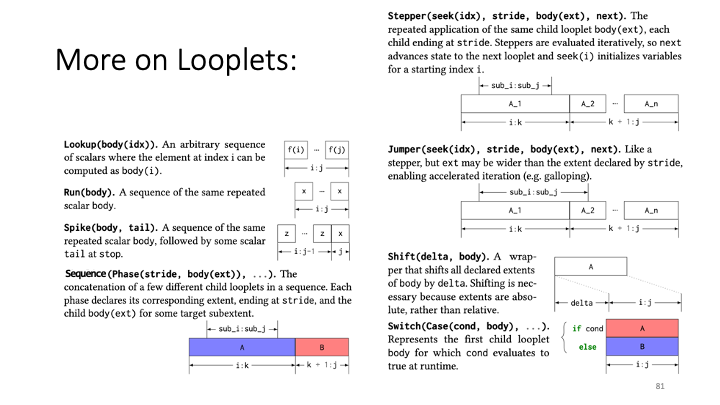
\includegraphics[width=\linewidth]{example_looplet_figure.png}
    \caption{Looplets visualized, along with their semantics}
\end{figure}

\subsection{FiberTrees}

\subsection{Concordant Iteration}

\subsection{Protocols}